
%is highly influential. Furthermore, It can be seen that features that describe the map density (ObstacleDensity, PointsAtSPRatio, Sparsity, AvgStartDistances, AvgGoalDistances) have high impact also. Yet, some features, those describing the grid (rows and columns) and other quantitative measures (number of obstacles, branching factor) were not as helpful.

%Using TreeExplainer method, we compute the Shapley value for each feature at every sample on all labels. In order to gain a global understanding of the impact each feature made on the model, we do the following steps:1. Compute the mean impact each feature had on the labels for every sample. 2. Compute the mean impact each feature had on all samples.[[Roni: I dont get step one: the model gives a single label to every sample]

%Further information on techniques about interpretable machine learning has been recently made \cite{du2018techniques}. In order to compute the importance of each feature to the model, we used \textit{TreeExplainer} method, as defined by \cite{lundberg2019explainable}. \textit{TreeExplainer} is based on a local explanation method, thus combining local explanations from many samples in order to gain global model insights. The local explanations computed based on SHapley Additive exPlanation (SHAP) values (\cite{lundberg2017unified}). The basic intuition of how to compute \textit{Shapely} values is to find the average of the marginal contributions across all permutations for a given feature. Further information on techniques about interpretable machine learning has been recently made \cite{du2018techniques}.Using TreeExplainer method, we compute the Shapley value for each feature at every sample on all labels. In order to gain a global understanding of the impact each feature made on the model, we do the following steps:1. Compute the mean impact each feature had on the labels for every sample.2. Compute the mean impact each feature had on all samples.

\begin{figure}[h]
    \centering
    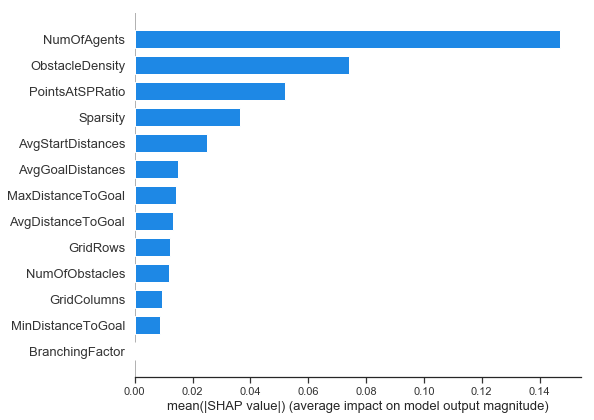
\includegraphics[width=0.5\textwidth]{Charts/mean_all_classes.png}
    \caption{Feature importance calculated using Shapley values. Features are sorted by their importance at y-axis. X-axis is the mean impact on model output, i.e. mean probability impact.}
    \label{fig:FeatureImportance}
\end{figure}

We can see that, as expected, the number of agents is highly influential. 
Furthermore, It can be seen that features that describe the map density (ObstacleDensity, PointsAtSPRatio, Sparsity, AvgStartDistances, AvgGoalDistances) have high impact also. 
Yet, some features, those describing the grid (rows and columns) and other quantitative measures (number of obstacles, branching factor) were not as helpful.

% As described above, our regression model consists of K regression models (where K is the number of algorithms, i.e. K=6). Here, we describe the feature importance for each regression model and use the results to enhance current assumptions about the different MAPF solvers we used.





\begin{center}
\begin{table}[t]
% Please add the following required packages to your document preamble:
% \usepackage{booktabs}
\centering
\resizebox{0.6\columnwidth}{!}{
\begin{tabular}{@{}lrrr@{}}
\toprule
Model                    & Accuracy & Coverage & Total RT \\ \midrule
 \astar+OD+ID & 0.00 & 0.73 & 12,459 \\
 EPE\astar & 0.12 & 0.79 & 9,871 \\ 
 ICTS & 0.10	& 0.78 & 10,570 \\
 CBS & 0.00 & 0.59 & 17,447 \\
 MA-CBS & 0.26 & 0.53	& 19,952 \\
 CBS-H & 0.50 & 0.83 & 8,016 \\ 
 \midrule
 Random & 0.16 & 0.71 & 13,215 \\  
 CNN Rg. & 0.51 & 0.88 & 6,210 \\ 
 XGBoost Rg. & 0.51	& 0.82 & 8,410 \\
 CNN Cl. & 0.55 & 0.91 & 5,122 \\
 XGBoost Cl. & 0.66 & 0.93 & 4,307 \\
 \midrule
 Oracle & 1.00 & 100.00 & 1,649 \\
\bottomrule
\end{tabular}
}
\caption{Results for all models across all the test set.}
\label{table:allResults}
\end{table}
\end{center}
\Roni{Maybe add another decimal point}





\begin{figure}
\centering
    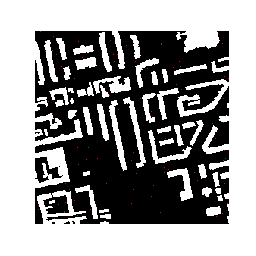
\includegraphics[width=0.75\linewidth]{images/Berlin_1_256-71-5-label1.png}
    \caption{A MAPF problem represented as images. Red and green pixels are source and target vertices of the agents.}
\label{fig:cnn-image}
\end{figure}


\begin{figure}
    \centering
    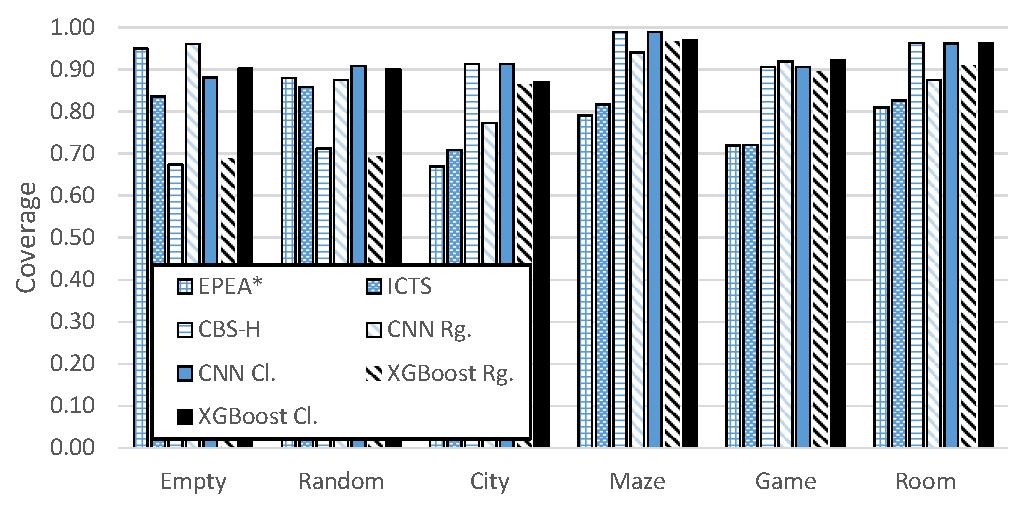
\includegraphics[width=\columnwidth]{coverageByMap.pdf}
    \caption{Coverage results, split by grid types.}
    \label{fig:coverageByMap}
\end{figure}